\documentclass[a4paper,10pt]{article}
\usepackage[utf8]{inputenc}
\usepackage{graphicx}
\usepackage{amsmath}
\usepackage{amssymb}
\usepackage{amsthm}
\usepackage{booktabs}
\usepackage{caption}
\usepackage{geometry}
%\usepackage{hyperref}
\usepackage{makeidx}
\usepackage{microtype}
\usepackage{subfig}
\usepackage{tabularx}
\usepackage{url}
\usepackage{varioref}
\usepackage{xcolor}
\usepackage{multicol}
\usepackage[italian]{babel}
\usepackage{mathtools}
\usepackage{booktabs}
\usepackage{multirow}
\usepackage{gensymb}


%%%%%%%%%%%%%%%%%%%%%%%%%%%%%%%%%%%%%%%%%%%%


\title{Laboratorio I: Misure di densità\\
\begin{large}
Dipartimento di Fisica E.Fermi - Università di Pisa
\end{large}}

\author{Di Ubaldo Gabriele}
\date{11 Novembre 2015}

\begin{document}

\maketitle


%%%%%%%%%%%%%%%%%%%%%%%%%%%%%%%%%%%%%%%%%%%%%%%%%%%%%%
\section{Introduzione}
\subsection{Teoria}
\textbf{Obbietivo:}Calcolare la densità di diversi solidi attraverso misure di volume e di massa e mostrare che vi è una dipendenza lineare tra queste potendo distinguere diversi materiali.

Definiamo la densità come la massa per unità di volume:

 \begin{equation}
    \rho=\frac{m}{V}
 \end{equation}

\begin{table}[!htb]
\centering
\caption{Densità attese}
\label{my-label}
\begin{tabular}{c|c|c}
\hline
Materiali            & \multicolumn{2}{l|}{Densità($kg/m^3$)} \\ \hline
Alluminio            & \multicolumn{2}{l|}{2710}                            \\ \hline
Acciaio inossidabile & \multicolumn{2}{l|}{7480-8000}                       \\ \hline
Ottone (lega Cu-Zn)  & \multicolumn{2}{l|}{8400-8700}                       \\ 



\end{tabular}
\end{table}


\subsubsection{Apparato sperimentale}
\begin{itemize}
 \item {Calibro ventesimale di risoluzione $0.05mm$}
 \item {Calibro Palmer $0.01mm$}
 \item {Bilancia di precisione $1g$}
 \item {Una serie di solidi in alluminio, acciao e ottone} 
\end{itemize}


%%%%%%%%%%%%%%%%%%%%%%%%%%%%%%%%%%%%%%%%%%%%%%%%%%%%%%%%%%%%%%%%%%%%%%%%%%%%%%%%%%%%%%%%%%%%%%
\section{Esperimento}
Disponiamo di 4 cilindri, 5 sfere, e 4 parallelepipedi; misuriamo i cilindri ed i parallelepipedi con il calibro ventesimale, in particolare misuriamo il diametro e le altezze per
i cilindri, per i parallelepipedi misuriamo i lati A, B, e C.
Per le sfere utilizziamo il calibro Palmer al fine di ottenere una maggiore precisione, misurando il diametro.
In seguito pesiamo i vari corpi e in fine calcoliamo la densità con il relativo errore.
\textit{\textbf{Dato che queste sono misure dirette, l'errore è lo stesso per tutte; in particolare le masse hanno un errore di $\pm0.001g$ e le altre lunghezze di $\pm 0.05cm$}}.
\begin{table}[!htb]
\centering
\caption{Misure}
\label{my-label}
\begin{tabular}{c|c|c|c|c|c}

\hline
    Solidi        & Massa (g) & Raggio (cm)     & Lato a (altezza)   & Lato b   & Lato c  \\ \hline
Parallelepipedo 1 & 28.821    & \textemdash & 17.7               & 7.5      & 8.5     \\ \hline
Parallelepipedo 2 & 34.672    & \textemdash & 41.6               & 10       & 10      \\ \hline
Parallelepipedo 3 & 4.864     & \textemdash & 10.15              & 17.6     & 10.15   \\ \hline
Parallelepipedo 4 & 8.004     & \textemdash & 20                 & 18.3     & 8.15    \\ 
Cilindro 2        & 24.725    & 5.00            & 37.65              & \textemdash & \textemdash \\ \hline
Cilindro 3        & 1.471     & 3.00            & 19.50              & \textemdash & \textemdash \\ \hline
Cilindro 4        & 15.673    & 9.80            & 18.80              & \textemdash & \textemdash \\ \hline
Sfera 1           & 3.528     & 4.75            & \textemdash & \textemdash & \textemdash \\ \hline
Sfera 2           & 8.365     & 6.35            & \textemdash & \textemdash & \textemdash \\ \hline
Sfera 3           & 11.894    & 7.15            & \textemdash & \textemdash & \textemdash \\ \hline
Sfera 4           & 18.914    & 8.32            & \textemdash & \textemdash & \textemdash \\ \hline
Sfera 5           & 24.830    & 9.15            & \textemdash & \textemdash & \textemdash \\ \hline
\end{tabular}
\end{table}
%%%%%%%%%%%%%%%%%%%%%%%%%%%%%%%%%%%%%%%%%%%%%%%%%%%%%%%%%%%%%%%%%%%%%%%%%%%%%%%%%%%%%%%%%%%%%%%%%%%%%%%%%

\section{Analisi dati}
Successivamente alla presa dati, possiamo utilizzare la formula della densità e tracciare un grafico del volume rispetto alla massa, aspettandoci un dipendenza lineare.In seguito andremo a 
calcolare il coefficiente angolare dal quale potremo ricavare la densità osservata dalle misure per poi confrontarla con le densità attesa.
Supponendo essere le misure indipendenti possiamo propagare l'errore sulla densità tramite la somma in quadratura, la quale fornisce un errore più esatto. Per calcolare i volumi sono state usate le corrispondenti formule di geometria su cui abbiamo propagato l'errore utilizzando lo sviluppo di Taylor in più variabili attraverso derivate parziali. Per esempio per cilindro e sfera si ha:
\begin{equation}
V_{cil}=\pi r^2  h \quad V_{sf}=\frac{4}{3}  \pi  r^3
\end{equation}

\begin{equation}
 \Delta V_{cil}=((2 \pi  r  h)  \frac{\Delta r}{r}  (\pi  r^2)  \frac{\Delta h}{h}) \quad \Delta V_{sf}=4  \pi  r^2  \frac{\Delta r}{r}
\end{equation}

Considerando i solidi che si supponeva fossero fatti dello stesso materiale, abbiamo fatto dei grafici del volume in funzione della massa secondo:
\begin{equation}
 V=\frac{1}{\rho}  m
\end{equation}
e li abbiamo fittati con Gnuplot (algoritmo di Marquardt-Levenberg)
\textbf {Alluminio}

\begin{table}[!htb]
\centering
\caption{Volume solidi alluminio}
\label{my-label}
\begin{tabular}{c|c|c}
\hline
                  & $V (cm^3)$ & $\sigma$ \\ \hline
Cilindro 3        & 551.35       & 19.79  \\ \hline
Cilindro 4        & 5672.31      & 72.96  \\ \hline
Parallelepipedo 3 & 3385         & 52     \\ \hline
Parallelepipedo 4 & 2982.9       & 33.9   \\ 
\end{tabular}
\end{table}
Per l'alluminio abbbiamo ottenuto un $\chi^2= 3.84$ con 3 gradi di libertà e dunque un $\tilde\chi^2=1.28$.
Otteniamo, infine, la stima di $\rho_{alluminio}=(2706 \pm 21)kg/m^3$.\\
\begin{figure}[!htb]
\begin{center}
 \centering 
 \caption{Grafico alluminio}
 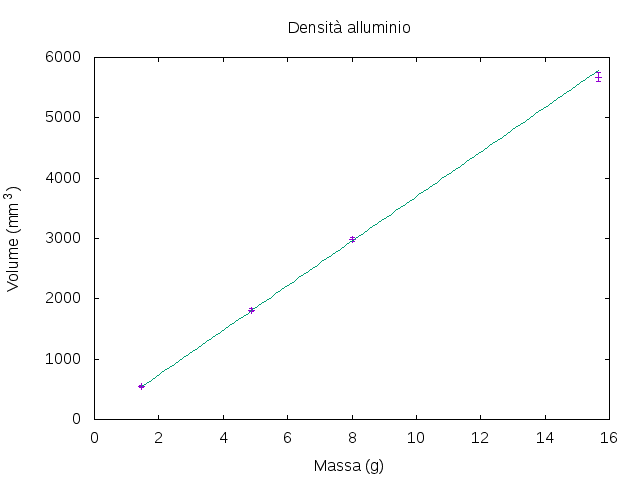
\includegraphics[width=11cm]{/home/zerch/Documents/UNIPI/LAB1/3Densita/Grafici/Grafico alluminio.png}
 \end{center}
\end{figure}
%%%%%%%%%%%%%%%%%%%%%%%%%%%%%%%%%%%%%%%%%%%%%%%%%%%%%%%%%%%%%%%%%%%%%%%%%
\textbf{Acciaio}
\begin{table}[!htb]
\centering
\caption{Volume solidi acciao}
\label{my-label}
\begin{tabular}{c|c|c}
\hline
                  & $V(cm^3)$ & $\sigma$  \\ \hline
Sfera 1           & 448.2        & 14.1   \\ \hline
Sfera 2           & 1072.5       & 25.3   \\ \hline
Sfera 3           & 1531.1       & 32.1   \\ \hline
Sfera 4           & 2416.8       & 43.5   \\ \hline
Sfera 5           & 3208.9       & 52.6   \\ \hline
\end{tabular}
\end{table}


Per l'acciaio abbiamo ottenuto un $\chi^2=50.15$ con 5 gradi di libertà e dunque un $\tilde\chi^2=10.29$.
Un risultato che può essere giustificato da una sottostima dell'errore sul cilindro 2.
Otteniamo la stima di $\rho_{acciao}=(7671 \pm 213)kg/m^3$.
\begin{figure}[!htb]
 \centering
 \caption{Grafico acciaio}
  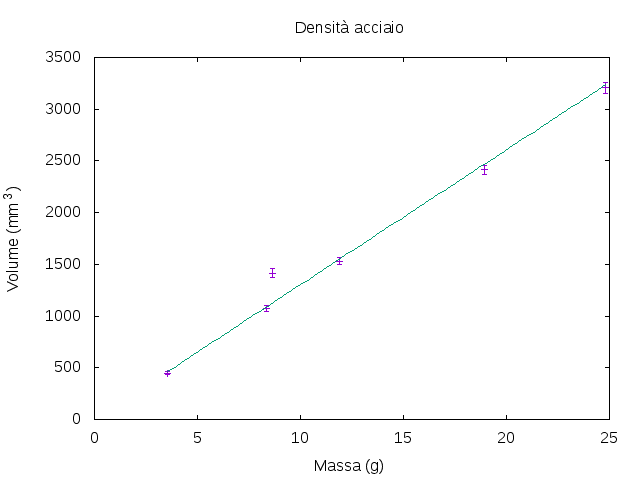
\includegraphics[width=11cm]{/home/zerch/Documents/UNIPI/LAB1/3Densita/Grafici/Grafico acciaio.png}
\end{figure}
%%%%%%%%%%%%%%%%%%%%%%%%%%%%%%%%%%%%%%%%%%%%%%%%%%%%%%%%%%%%%%%%%%%%%%%%%%
\textbf{Ottone}
\begin{table}[!htb]
\centering
\caption{Volumi solidi ottone}
\label{my-label}
\begin{tabular}{c|c|c}
\hline
                   & $V(cm^3)$ & $\sigma$ \\ \hline
Cilindro 2         & 2957.02                       & 63.06  \\ \hline
Parallelepipedo 1  & 3385                          & 52     \\ \hline
Paralleleppipedo 2 & 4160                          & 37     \\ 
\end{tabular}
\end{table}\\\\\\
Per l'ottone otteniamo un $\chi^2=1.15$ con 2 gradi di libertà ed un $\tilde\chi^2=0.6$.
Otteniamo la stima di $\rho_{ottone}=(8396 \pm 46)kg/m^3$.
\begin{figure}[!htb]
\begin{center}
\centering 
\caption{Grafico ottone}
  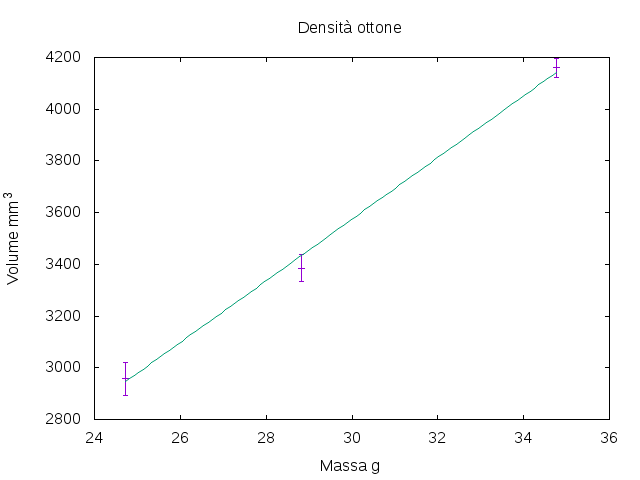
\includegraphics[width=11cm]{/home/zerch/Documents/UNIPI/LAB1/3Densita/Grafici/Grafico ottone.png}
\end{center}
\end{figure}
%%%%%%%%%%%%%%%%%%%%%%%%%%%%%%%%%%%%%%%%%%%%%%%%%%%%%%%%%%%%%%%%%%%%%%%%%%
%%%%%%%%%%%%%%%%%%%%%%%%%%%%%%%%%%%%%%%%%%%%%%%%%%%%%%%%%%%%%%%%%%%%%%%%%%%%%%%%%%%%%%%%%%%%%%%%%%%%%%%%%%%%
\subsection{Legge di scala per le sfere}
Vi è una dipendenza cubica tra la massa e il raggio delle sfere che possiamo verificare tramite un grafico in carta bilogaritmica. Dovremmo ottenere una retta con coefficiente angolare 3 e intercetta $4\pi\rho/3$.
Abbiamo fittato con $y=Ax^B$ dove 
\begin{equation}
 A=\frac{4}{3} \times \pi \times \rho_{acc}=32132 \pm 101 kg/m^3
\end{equation}

\begin{table}[!htb]
\centering
\caption{Masse e raggi}
\label{my-label}
\begin{tabular}{|l|l|l|}
\hline
        & Massa (g)     & Raggio (cm) \\ \hline
Sfera 1 & 3.528+-0.001  & 4.75+-0.05  \\ \hline
Sfera 2 & 8.365+-0.001  & 6.35+-0.005 \\ \hline
Sfera 3 & 11.894+-0.001 & 7.15+-0.05  \\ \hline
Sfera 4 & 18.914+-0.001 & 8.32+-0.05  \\ \hline
Sfera 5 & 24.830+-0.001 & 9.15+-0.05  \\ \hline
\end{tabular}
\end{table}
\begin{figure}[!htb]
\begin{center}
 \centering
 \caption{Sfere}
 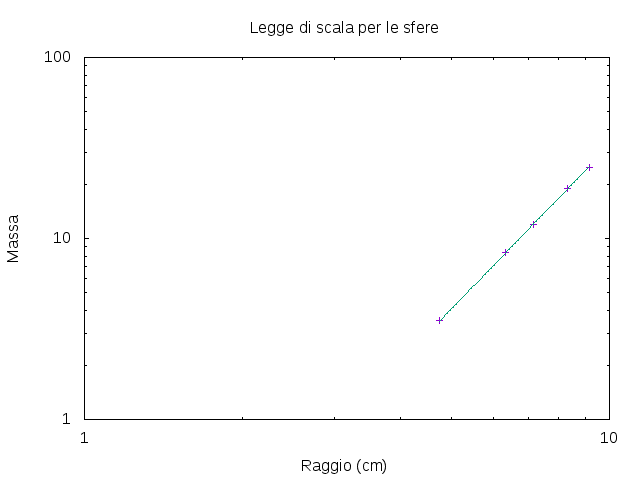
\includegraphics[width=11cm]{/home/zerch/Documents/UNIPI/LAB1/3Densita/Grafici/Grafico sfere.png}
 \end{center}
\end{figure}
Qui riportiamo il grafico della massa in funzione del raggio e vediamo che $B=2.98 \pm 0.02$ il che rispecchia il valore atteso, inceve vediamo che interseca l'asse delle x
e corrisponde al valore del raggio che deve possedere una sfera di massa 1g è: $r=\sqrt[3]{\frac{3  1}{4  \rho}}=(3.05 \pm 0.01)mm$.
Da ciò otteniamo, andando a sostituire nella (14), il seguente valore: $A=\frac{y}{r^3}=(35245 \pm 107)kg/m^3$, in concordanza con la A calcolata precedentemente.
%%%%%%%%%%%%%%%%%%%%%%%%%%%%%%%%%%%%%%%%%%%%%%%%%%%%%%%%%%%%%%%%%%%%%%%%%%%%%%%%%%%%%%%%%
\section{Conclusione}
Possiamo concludere affermando che le misure delle densità tabulate sono corripondenti alle densità da noi misurate entro il relativo errore.
Inoltre dallo studio del grafico e dalle considerazioni fatte sulla legge di potenza delle sfere possiamo concludere che vi è un una certa dipendenza.
\end{document}
